
\section{Caf� Gumbel}

Das Caf� Gumbel ist ein vor Jahrzehnten erstreikter Aufenthalts- und Lernraum mit Teek�che.  Das Gumbel wird von Studierenden betrieben.  W�hrend der
�ffnungszeiten ist der Raum inklusive K�che mit Wasserkocher und Geschirr
jedem zug�nglich.

Falls du gerne einen Poetry Slam, Spieleabend oder
eine andere Veranstaltung f�r dich und deine Kommilitonen organisieren
m�chtet, frag einfach an.  Wir stellen euch gerne einen Beamer, Soundanlage,
Spielkarten (usw.) zur Verf�gung.

Theresienstr., B030\\
Mo -- Fr: 8:00 -- 22:00~Uhr (meistens)\\
Kontakt: \url{gumbel@fs.lmu.de}

\skiptobottom
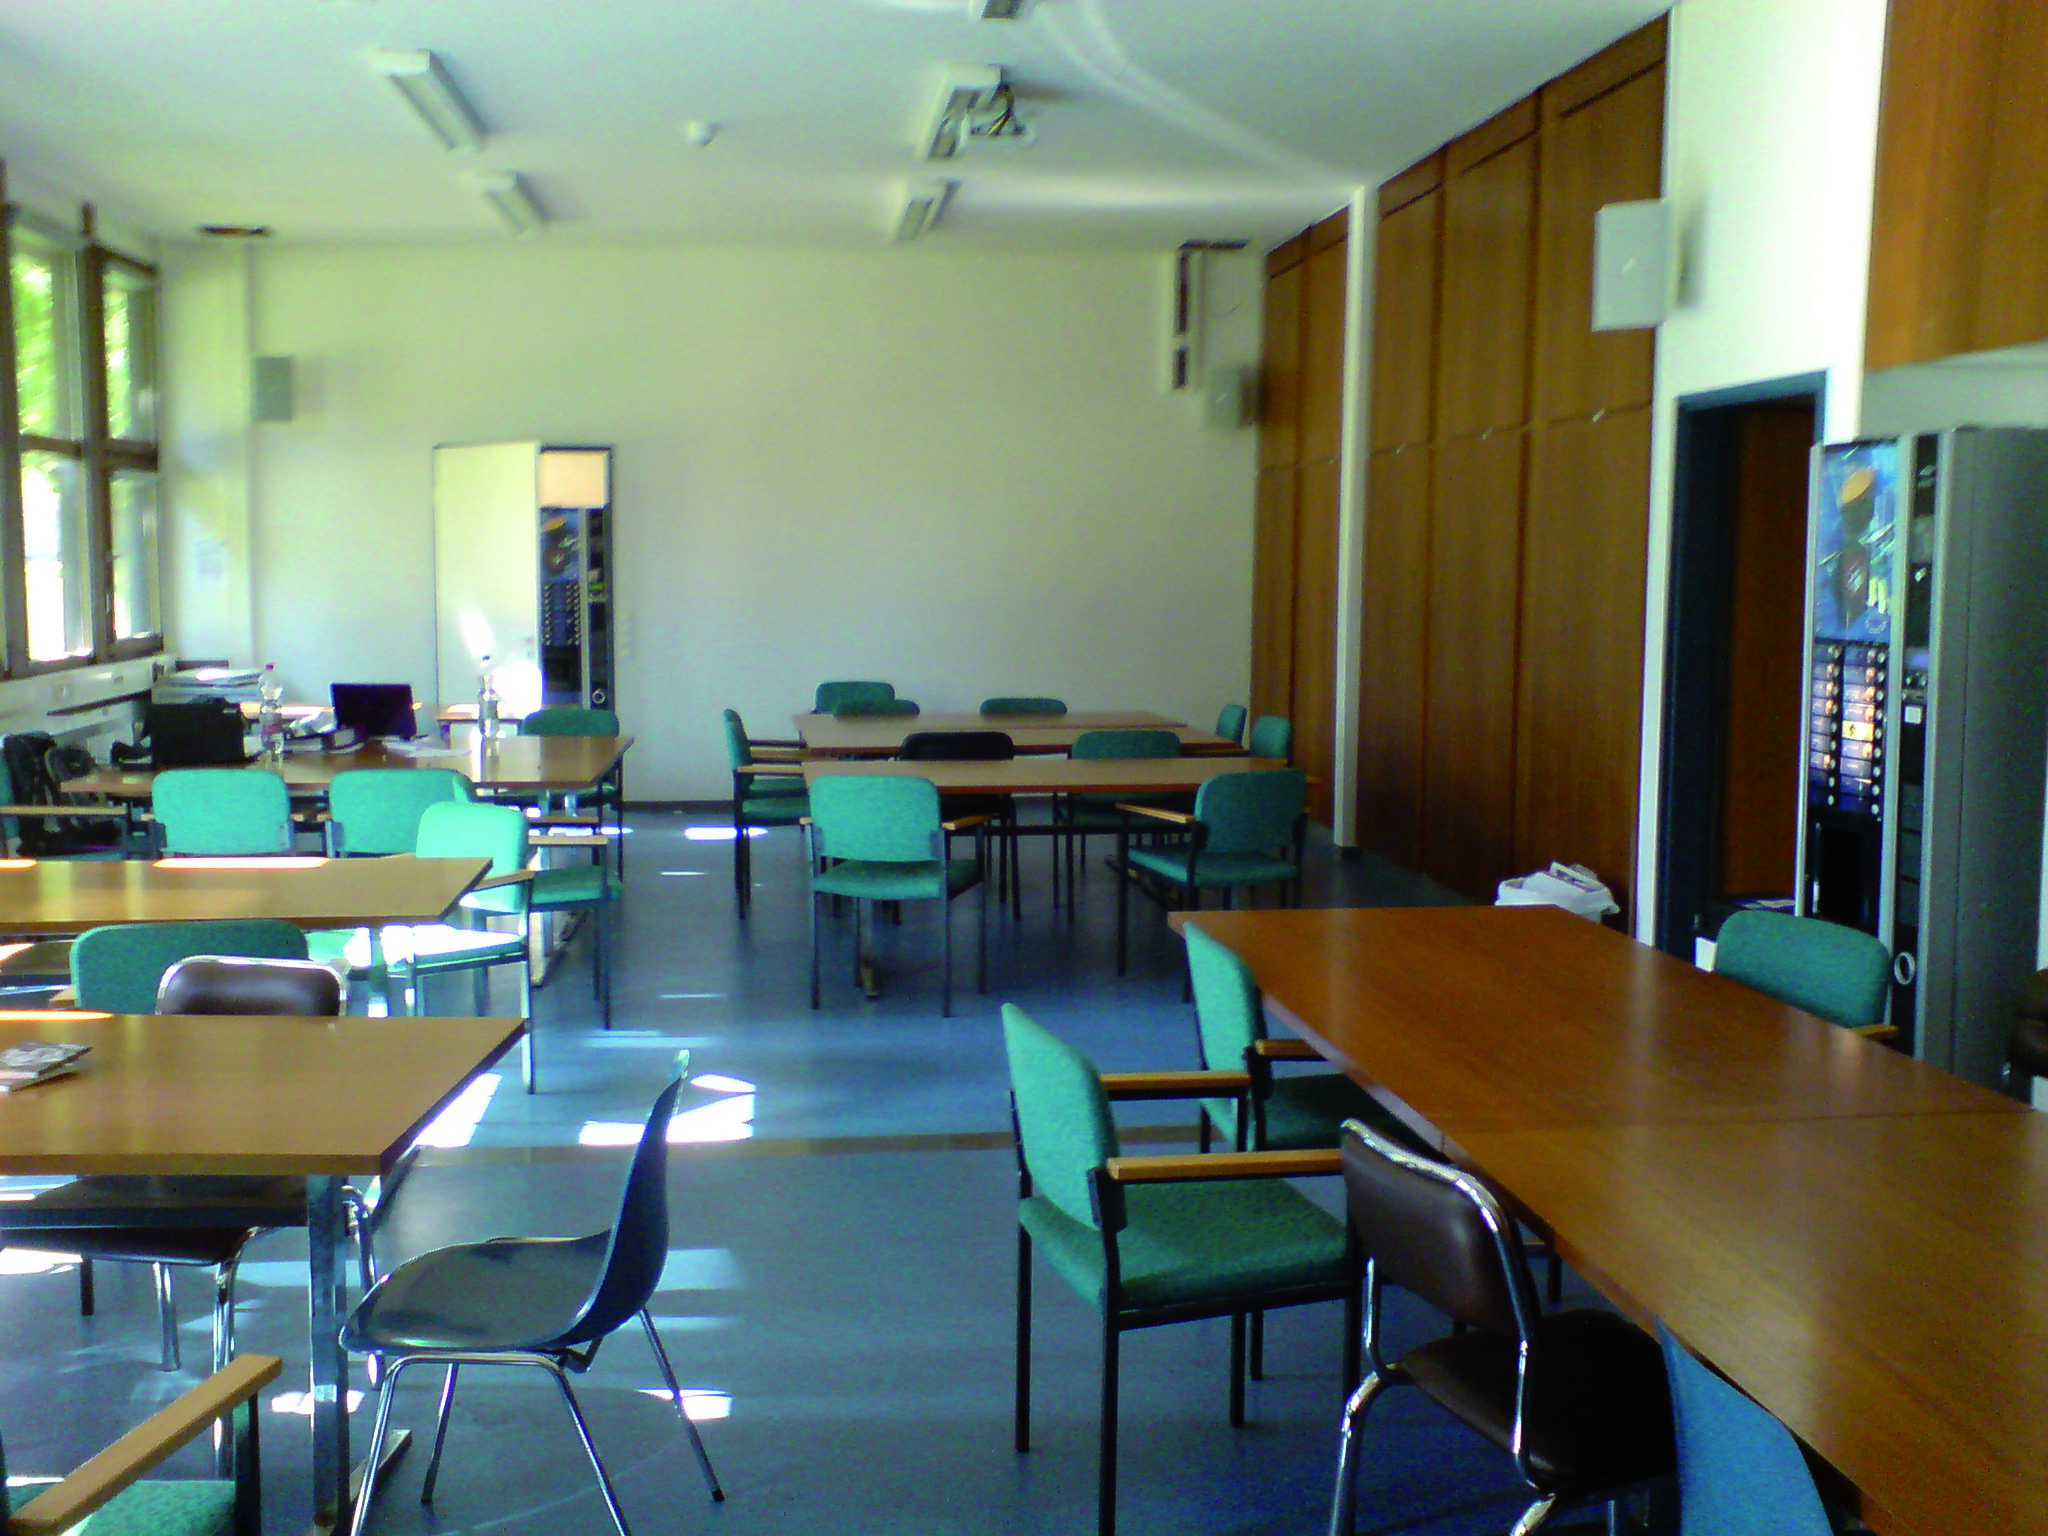
\includegraphics[width=\textwidth]{gumbel_raum_print}
